\documentclass[border=6pt]{standalone}
\usepackage{amsmath}
\usepackage{amssymb}
\usepackage{tikz}
\usetikzlibrary{arrows.meta,calc,decorations.pathreplacing,patterns,shapes.geometric,positioning,shadings,plotmarks}

\begin{document}
\begin{tikzpicture}[scale=1.0,>={Latex[length=2mm]}]

% =========================================================================
% van der Waals isotherms in reduced units (V = v/v_c, P = p/p_c, T = T/T_c)
% Reduced equation:  P = 8 T / (3 V - 1) - 3 / V^2
% Critical point:    (V, P) = (1, 1)
%
% Plot scaling:
%   x = xs * V,   y = ys * P
% so the plotting box is roughly 0..xs*Vmax  by  0..ys*Pmax
% =========================================================================

\def\xs{2.4}     % horizontal scale
\def\ys{3.6}     % vertical scale
\def\Vmax{4.6}   % max reduced volume to display
\def\Pmax{1.85}  % max reduced pressure to display

% -------------------------------------------------------------------------
% Maxwell construction at T_r = 0.9 (numerically pre-computed)
%   P_sat ~= 0.6470
%   V_l   ~= 0.6033  (liquid)
%   V_g   ~= 1.7472  (gas)
%   middle root V_m ~= 0.8631 (curve crosses P_sat between extrema)
%   local minimum at V ~= 0.6845 (P_min ~= 0.5828)  <-- left extremum
%   local maximum at V ~= 1.7268 (here actually P_max barely above P_sat;
%                                  we use V_lmax ~= 1.45 for visual unstable end)
% Actually for T_r = 0.9 the local max sits at V ~= 1.722 (just inside V_g),
% and local min at V ~= 0.685. We use these for the dashed (unstable) segment.
% -------------------------------------------------------------------------

\def\Psat{0.6470}
\def\Vl{0.6033}
\def\Vg{1.7472}
\def\Vm{0.8631}      % middle root: curve = P_sat between extrema
\def\Vlmin{0.6845}   % local min of P(V) at T_r=0.9
\def\Vlmax{1.4500}   % visual right end of unstable (S-curve) region

% =========================================================================
% (1) Shaded equal-area regions  --  drawn first, behind curves
% =========================================================================

% Region A_up : curve ABOVE horizontal line, V in [V_l, V_m]
% Bounded above by the vdW isotherm, below by P = P_sat
\fill[orange!35,opacity=0.7]
  plot[domain=\Vl:\Vm,samples=70,smooth]
    ({\xs*\x}, {\ys*( 8*0.9/(3*\x - 1) - 3/(\x*\x) )})
  -- ({\xs*\Vm}, {\ys*\Psat})
  -- ({\xs*\Vl}, {\ys*\Psat}) -- cycle;

% Region A_down : curve BELOW horizontal line, V in [V_m, V_g]
% Bounded above by P = P_sat, below by the vdW isotherm
\fill[orange!35,opacity=0.7]
  ({\xs*\Vm}, {\ys*\Psat}) --
  plot[domain=\Vm:\Vg,samples=90,smooth]
    ({\xs*\x}, {\ys*( 8*0.9/(3*\x - 1) - 3/(\x*\x) )})
  -- ({\xs*\Vg}, {\ys*\Psat}) -- cycle;

% =========================================================================
% (2) Coordinate axes
% =========================================================================
\draw[->,gray!75,thick] (0,0) -- ({\xs*\Vmax + 0.4}, 0) node[right,black]{$v$};
\draw[->,gray!75,thick] (0,0) -- (0, {\ys*\Pmax + 0.3}) node[above,black]{$p$};
\node[below left,black] at (0,0) {$O$};

% =========================================================================
% (3) High-temperature isotherm  T_r = 1.30  (blue, monotonic)
% =========================================================================
\draw[blue!70!black,very thick,smooth,samples=140,domain=0.40:\Vmax]
  plot ({\xs*\x}, {\ys*( 8*1.30/(3*\x - 1) - 3/(\x*\x) )});

% =========================================================================
% (4) Critical isotherm  T_r = 1.0  (black, horizontal inflection at (1,1))
% =========================================================================
\draw[black,very thick,smooth,samples=160,domain=0.40:\Vmax]
  plot ({\xs*\x}, {\ys*( 8*1.0/(3*\x - 1) - 3/(\x*\x) )});

% =========================================================================
% (5) Low-temperature isotherm  T_r = 0.9  (brick red, S-shape)
%     -- middle (unstable) segment dashed; rest solid
% =========================================================================

% Solid: from small V up to local minimum
\draw[red!60!black,very thick,smooth,samples=80,domain=0.42:\Vlmin]
  plot ({\xs*\x}, {\ys*( 8*0.9/(3*\x - 1) - 3/(\x*\x) )});

% Dashed: unstable region V_lmin .. V_lmax  (dp/dv > 0, non-physical)
\draw[red!60!black,very thick,dashed,smooth,samples=80,domain=\Vlmin:\Vlmax]
  plot ({\xs*\x}, {\ys*( 8*0.9/(3*\x - 1) - 3/(\x*\x) )});

% Solid: from local maximum out to large V
\draw[red!60!black,very thick,smooth,samples=120,domain=\Vlmax:\Vmax]
  plot ({\xs*\x}, {\ys*( 8*0.9/(3*\x - 1) - 3/(\x*\x) )});

% =========================================================================
% (6) Maxwell horizontal segment  P = P_sat  from V_l to V_g
% =========================================================================
\draw[red!60!black,thick,dashed]
  ({\xs*\Vl}, {\ys*\Psat}) -- ({\xs*\Vg}, {\ys*\Psat});

% =========================================================================
% (7) Critical point  (V_c, P_c) = (1, 1)
% =========================================================================
\fill[red] ({\xs*1.0}, {\ys*1.0}) circle (2.4pt);
\node[above right=1pt and 1pt,font=\small] at ({\xs*1.0}, {\ys*1.0}) {$(v_c,p_c)$};

% =========================================================================
% (8) Liquid / gas endpoints (filled dots) + vertical/horizontal guides
% =========================================================================
\fill[black] ({\xs*\Vl}, {\ys*\Psat}) circle (1.8pt);
\fill[black] ({\xs*\Vg}, {\ys*\Psat}) circle (1.8pt);

% Vertical guide lines  v_l, v_g, v_c
\draw[gray!55,densely dotted] ({\xs*\Vl}, 0) -- ({\xs*\Vl}, {\ys*\Psat});
\draw[gray!55,densely dotted] ({\xs*\Vg}, 0) -- ({\xs*\Vg}, {\ys*\Psat});
\draw[gray!55,densely dotted] ({\xs*1.0}, 0) -- ({\xs*1.0}, {\ys*1.0});
\node[below,font=\small] at ({\xs*\Vl}, 0) {$v_l$};
\node[below,font=\small] at ({\xs*\Vg}, 0) {$v_g$};
\node[below,font=\small] at ({\xs*1.0}, 0) {$v_c$};

% Horizontal guide lines  p_sat, p_c
\draw[gray!55,densely dotted] (0, {\ys*\Psat}) -- ({\xs*\Vl}, {\ys*\Psat});
\draw[gray!55,densely dotted] (0, {\ys*1.0}) -- ({\xs*1.0}, {\ys*1.0});
\node[left,font=\small] at (0, {\ys*\Psat}) {$p_{\mathrm{sat}}$};
\node[left,font=\small] at (0, {\ys*1.0}) {$p_c$};

% =========================================================================
% (9) Isotherm labels (placed near the right edge of each curve)
% =========================================================================
% T > T_c  (blue): at V=4.2, the curve sits at P ~= 8*1.3/(12.6-1) - 3/17.64 = 0.897 - 0.170 = 0.727
\node[blue!70!black,font=\small,right] at ({\xs*4.2}, {\ys*0.78}) {$T>T_c$};

% T = T_c  (black): at V=4.2, P ~= 8/(11.6) - 3/17.64 = 0.690 - 0.170 = 0.520
\node[black,font=\small,right] at ({\xs*4.2}, {\ys*0.55}) {$T=T_c$};

% T < T_c  (red): at V=4.2, P ~= 8*0.9/(11.6) - 3/17.64 = 0.621 - 0.170 = 0.451
\node[red!60!black,font=\small,right] at ({\xs*4.2}, {\ys*0.32}) {$T<T_c$};

% =========================================================================
% (10) Area-region labels  A_up  (above the line)  and  A_down  (below)
% =========================================================================
\node[font=\small,black] at ({\xs*0.74}, {\ys*0.83}) {$A_{\uparrow}$};
\node[font=\small,black] at ({\xs*1.20}, {\ys*0.50}) {$A_{\downarrow}$};

% =========================================================================
% (11) van der Waals equation -- placed in empty top-right area
% =========================================================================
\node[draw=gray!55,fill=white,rounded corners=2pt,inner sep=4pt,font=\small]
  at ({\xs*3.4}, {\ys*1.55})
  {$\left(p+\dfrac{a}{v^{2}}\right)(v-b)=RT$};

% =========================================================================
% (12) Maxwell condition statement
% =========================================================================
\node[draw=orange!65,fill=orange!10,rounded corners=2pt,inner sep=4pt,
      font=\small,align=center]
  at ({\xs*3.4}, {\ys*1.15})
  {Maxwell: $A_{\uparrow}=A_{\downarrow}$\\[1pt]
   $\Longleftrightarrow\;\displaystyle \oint v\,\mathrm{d}p = 0$};

\end{tikzpicture}
\end{document}
